
\section{ICE} \label{Sec:ICE}


\subsection{Introduction}
\red{
finite volume
first order tempral discretizatioon
all speed
with the option of explicit or semi-implicit }

\subsection{Theory - Algorithm Description}

\subsection{Uintah Specification}
%______________________________________________________________________
\subsubsection{Basic Inputs}

Each Uintah component is invoked using a single executable called
\it sus \normalfont, which chooses the type of simulation
to execute based on the \it SimulationComponent \normalfont tag in the
input file.  In the case of ICE simulations, this looks like:

\begin{Verbatim}[fontsize=\footnotesize]
 <SimulationComponent type="ice" />
\end{Verbatim}

%______________________________________________________________________
\subsubsection{Physical Constants}

\begin{Verbatim}[fontsize=\footnotesize]
<PhysicalConstants>
   <gravity>            [0,0,0]   </gravity>
   <reference_pressure> 101325.0  </reference_pressure>
</PhysicalConstants>
\end{Verbatim}

%______________________________________________________________________
\subsubsection{Material Properties}
For each ICE material the thermodynamic and transport properties must be
specified, in addition to the initial conditions of the fluid inside of
each geom\_object.  Below is the an example of how to specify an invisid
ideal gas over square region with dimensions $6m X 6m X 6m$.  The initial
conditions of the gas in that region are $T=300, \rho=1.179, v_x=1,v_y=2,
v_z=3$ \big{(}Note, the pressure XML tag is not used as an initial condition
and is simply there to make the user aware of what the pressure would be at
that thermodynamic state.\big{)}
%
\begin{Verbatim}[fontsize=\footnotesize]
<MaterialProperties>
   <ICE>
     <material>
       <EOS type = "ideal_gas">                     </EOS>
       <dynamic_viscosity>   0.0                    </dynamic_viscosity>
       <thermal_conductivity>0.0                    </thermal_conductivity>
       <specific_heat>      716.0                   </specific_heat>
       <gamma>              1.4                     </gamma>
       <geom_object>
           <box label="wholeDomain">
               <min>       [ 0.0, 0.0, 0.0 ]       </min>
               <max>       [ 6.0, 6.0, 6.0 ]       </max>
           </box>
           <res>                 [2,2,2]            </res>
           <velocity>      [1.,2.,3.]               </velocity>
           <density>       1.1792946927374306000e+00</density>
           <pressure>      101325.0                 </pressure>     
           <temperature>   300.0                    </temperature>
       </geom_object>
     </material>
  </ICE>       
</MaterialProperties>
\end{Verbatim}
%______________________________________________________________________
\subsubsection{Equation of State}
Below is a list of the various equations of state, along with the user defined
constants, that are available.  The reader should consult the literature for
the theoretical development and applicability of the equations of state to
the problem being solved.
%
%
The most commonly used EOS is the ideal gas law
\begin{equation}
  p = (\gamma -1) c_v \rho T
\end{equation}
%
and is specified in the input file with:
%
\begin{Verbatim}[fontsize=\footnotesize]
<EOS type="ideal_gas"/>
\end{Verbatim}
%
The Thomsen Hartka EOS for cold liquid water (1-100 atm pressure range)
is specified with \cite{ref:Thomsen,ref:bejan}
%
\begin{Verbatim}[fontsize=\footnotesize]
<EOS type="Thomsen_Hartka_water">
  <a>  2.0e-7     </a>    <!-- (K/Pa)     -->    
  <b>  2.6        </b>    <!-- (J/kg K^2) -->
  <co> 4205.7     </co>   <!-- (J/Kg K)   -->
  <ko> 5.0e-10    </ko>   <!-- (1/Pa)     -->
  <To> 277.0      </To>   <!-- (K)        -->
  <L>  8.0e-6     </L>    <!-- (1/K^2)    -->
  <vo> 1.00008e-3 </vo>   <!-- (m^3/kg)   -->
</EOS>
\end{Verbatim}
% 
%
The input specification for the ``JWLC'', ``JWL++'' and ``Murnahan'' equations of state from \cite{ref:JWL} are: 
\begin{Verbatim}[fontsize=\footnotesize]
<EOS type = "JWLC">
  <A>   2.9867e11   </A>
  <B>   4.11706e9   </B>
  <C>   7.206147e8  </C>
  <R1>    4.95      </R1>
  <R2>    1.15      </R2>
  <om>    0.35      </om>
  <rho0>  1160.0    </rho0>
</EOS>
\end{Verbatim}
%
\begin{Verbatim}[fontsize=\footnotesize]
<EOS type = "JWL">
  <A>     1.6689e12 </A>
  <B>     5.969e10  </B>
  <R1>      5.9     </R1>
  <R2>      2.1     </R2>
  <om>      0.45    </om>
  <rho0>  1835.0    </rho0>
</EOS>
\end{Verbatim}
%
\begin{Verbatim}[fontsize=\footnotesize]
<EOS type = "Murnahan">
  <n>     7.4       </n>
  <K>     39.0e-11  </K>
  <rho0>  1160.0    </rho0>
  <P0>    101325.0  </P0>
</EOS>
\end{Verbatim}
%
The ``hard sphere'' or ``Abel'' equation of state for dense gases is
%
\begin{equation}
  p(v - b) = RT
\end{equation}
%
where b corresponds to the volume occupied by the molecules themselves \cite{ref:thompson}.
Input parameters are specified using:
%
\begin{Verbatim}[fontsize=\footnotesize]
<EOS type="hard_sphere_gas">
   <b> 1.4e-3 </b>
</EOS>
\end{Verbatim}
%
%
Non-idea gas equation of state used in HMX combustion simulations the Twu-Sim-Tassone(TST) EOS
is
\begin{equation}
  p = \frac{ (\gamma -1)c_v T }{ v - b} - \frac{ a }{(v+3.0b)(v-0.5b)}
\end{equation}
%
Input parameters are specified using:
%
\begin{Verbatim}[fontsize=\footnotesize]
<EOS type="TST">
  <a>       -260.1385968     </a>
  <b>       7.955153678e-4   </b>
  <u>       -0.5             </u>
  <w>       3.0              </w>
  <Gamma>   1.63             </Gamma>
</EOS>
\end{Verbatim}
%
%
The input parameters for the Tillotson equation of state \cite{ref:gathers} for soils :
%
\begin{Verbatim}[fontsize=\footnotesize]
<EOS type = "Tillotson">
  <a>       .5      </a>
  <b>       1.3     </b>
  <A>       4.5e9   </A>
  <B>       3.0e9   </B>
  <E0>      6.e6    </E0>
  <Es>      3.2e6   </Es>
  <Esp>     18.0e6  </Esp>
  <alpha>   5.0     </alpha>
  <beta>    5.0     </beta>
  <rho0>    1700.0  </rho0>
</EOS>
\end{Verbatim}
%
%______________________________________________________________________
\subsubsection{Exchange Properties}
The heat and momentum exchange coefficients $K_{rs}$ and $H_{rs}$, which determine the rate at which momentum and heat are transferred between materials, are specified in the following format.
%
\begin{Verbatim}[fontsize=\footnotesize]
0->1,   0->2,  0->3
        1->2,  1->3
               2->3
\end{Verbatim}
%
For a two material problem the coefficients would be:
%
\begin{Verbatim}[fontsize=\footnotesize]
<exchange_properties> 
   <exchange_coefficients>
      <momentum>  [0, 1e15, 1e15 ]     </momentum>
      <heat>      [0, 1e10, 1e10 ]     </heat>  
   </exchange_coefficients>
</exchange_properties>
\end{Verbatim}
%
%
%______________________________________________________________________
\subsubsection{BoundaryConditions}
Boundary conditions must be specified on each face of the computational
domain $(x^-, x^+, y^-, y^+,z^-,z^+)$ for the variables $P, \bf{u}, T, \rho, v$ for
each material.  The three main types of numerical boundary conditions that can
be applied are ``Neumann",  ``Dirichlet" and ``Symmetric".  A Neumann boundary condition
is used to set the gradient or $\frac{\partial{q}}{\partial{n}}|_{surface} =
value$ at the boundary.   The value of the primative variable in the boundary
cell is given by,
%
\begin{equation}
    q[\text{boundary cell}] = q[\text{interior cell}] - value * dn;
\end{equation}
%
if we use a first order upwind discretization of the gradient.  Dirichlet boundary conditions set the value of primative variable in the boundary cell using
%
\begin{equation}
    q[\text{boundary cell}] =  value;
\end{equation}
%
\begin{Verbatim}[fontsize=\footnotesize]
<Grid>
  <BoundaryConditions>
    <Face side = "x-">
      <BCType id = "0"   label = "Pressure"     var = "Neumann">
                            <value> 0. </value>
      </BCType>
      <BCType id = "all" label = "Velocity"     var = "Neumann">
                            <value> [0.,0.,0.] </value>
      </BCType>
      <BCType id = "all" label = "Temperature"  var = "Neumann">
                            <value> 0.0 </value>
      </BCType>
      <BCType id = "all" label = "Density"      var = "Neumann">
                            <value> 0.0 </value>
      </BCType>
      <BCType id = "all" label = "SpecificVol"  var = "computeFromDensity">
                            <value> 0.0  </value>
      </BCType>
    </Face>
      .
      [other faces]
      .
  </BoundaryConditions>
</Grid>
\end{Verbatim}
Note that pressure field id is always 0. 
%
%
Symmetric boundary conditions are set using:
\begin{Verbatim}[fontsize=\footnotesize]
<Face side = "y-">
    <BCType id = "all" label = "Symmetric" var = "symmetry"> </BCType>
</Face>
\end{Verbatim}
%
\begin{center}
Boundary Condition Variables
\begin{tabular}{l p{7cm} p{7cm}}
\footnotesize{XML tag} & \footnotesize{Options}& \footnotesize{Description}\\
\hline
\hline
id          &  [0,1,2...all]                                   &   material index.\\
label       & [Temperature, Pressure, Density, SpecificVol]    &   primative variable name\\
var         & [Neumann, Dirichlet, symmetry]                   &   type of boundary condition to apply \\
value       & [ double or vector]                              &   "value" to be used when applying a BC\\
\hline
\end{tabular}
\end{center}
\normalsize
%______________________________________________________________________
\subsubsection{Semi-Implicit Pressure Solve}
The equation for the change in the pressure field $\Delta{P}$ during a given
timestep is given by
%
\begin{equation}
    \label{eq:delP}
     \frac{dP}{dt} = 
     \frac{\sum \limits_{{m}=1}^N  \frac{\dot{m}} {V \rho^{o}_m} 
        -  \sum \limits_{{m}=1}^N \nabla \cdot \widehat{\theta_m} \vec{U_m}^{*^{f}}}
          {\sum \limits_{{m}=1}^N \frac{\theta_m}{\rho^{o}_m c_m^2} }
\end{equation}
%
which can be written in matrix form $Ax = b$ and solved with a linear solver.  Details on the
notation, discretization of Eq. \ref{eq:delP} and the formation of $A$
and $b$ can be found in
%
\begin{Verbatim}[fontsize=\footnotesize]
 src/CCA/Components/ICE/Docs/implicitPressSolve.pdf
\end{Verbatim}
%
The linear system $Ax = b$ can be solved using the default Uintah:conjugate
gradient solver (CG) (slow) or using one of the many that are available
through the scalable linear solvers and preconditioner package hypre
\cite{ref:hypre}. Experience has shown that the most efficient hypre
preconditioner and solver are the pfmg and cg respectively.  Below are
typical values for both the Uintah:CG and hypre cg solver
%
\begin{Verbatim}[fontsize=\footnotesize]
<ImplicitSolver>
   <max_outer_iterations>         20    </max_outer_iterations>
   <outer_iteration_tolerance>    1e-8  </outer_iteration_tolerance>
   <iters_before_timestep_restart> 5    </iters_before_timestep_restart>
   <Parameters variable="implicitPressure">

    <tolerance>     1.e-10  </tolerance>
    
    <!-- CGSolver options -->
    <norm>     LInfinity  </norm>
    <criteria> Absolute   </criteria>

    <!-- Hypre options -->
    <solver>         cg      </solver>
    <preconditioner> pfmg    </preconditioner>
    <maxiterations>  7500    </maxiterations>
    <npre>           1       </npre>
    <npost>          1       </npost>
    <skip>           0       </skip>
    <jump>           0       </jump>
   </Parameters>
</ImplicitSolver>
\end{Verbatim}
%
If the user is interested in altering the tolerance to which the equations are solved they should look at
\begin{Verbatim}[fontsize=\footnotesize]
<tolerance> and <outer\_iteration\_tolerance>
\end{Verbatim} 
%
\noindent
\footnotesize
\begin{tabular}{l p{8cm}}
XML tag &  Description\\
\hline
\hline
max\_outer\_iterations           &  maximum number of iterations in the outer loop of the pressure solve.\\
outer\_iteration\_tolerance      &  tolerance XXXXDX\\
iters\_before\_timestep\_restart &  \footnotesize number of outer iterations before a timestep is restarted\\
tolerance                        &   XXXX\\
\hline
\end{tabular}
\normalsize\\
%
Table below shows some of the

\normalsize
%______________________________________________________________________
%  XML tags
\subsubsection{XML tag description}




%__________________________________
\begin {center}
\begin{tabular}{lllp{8cm}}
\\
\footnotesize{XML tag} & \footnotesize{Type} & \footnotesize{Dimensions} & \footnotesize{Description}\\
\hline
\hline
cfl                   & double &               &    Courant Number.\\
gravity               & Vector & $[L/t^2]$     &    gravitational acceleration, $\vec{g}$.\\
\\
\underline{\footnotesize{global material properties}} & & &\\
dynamic\_viscosity    & double & $[M/Lt]$      &    viscosity, $\mu$.\\
thermal\_conditucivity& double & $[ML/t^3T]$   &    thermal conductivity, $k$\\
specific\_heat        & double & $ [L^2/t^2 T]$ &   $c_p$\\
gamma                 & double &               &    ratio of specific heats, $\gamma$.\\
\\
\underline{\footnotesize{geometry object related}} & & &\\
res                   & vector &               &    resolution used for defining geometry objects.\\
velocity              & vector & $[L/t]$       &    initial velocity, $vec{u}$.\\
density               & double & $[M/L^3]$     &    initial density, $\rho$.\\
temperature           & double & $[T]$         &    initial temperature, $T$.\\
pressure              & double &               &    Not used. \\
\\
\underline{\footnotesize{AMR Parameters}} & & & \\
orderOfInterpolation  & integer &              &    Order of interpolation at the coarse/fine interfaces. \\
do\_Refluxing         & boolean &              &    on/off switch for correcting the flux of mass, momentum, and energy at the
                                                    course/fine interfaces.\\
\hline
\end{tabular}
\end{center}


%______________________________________________________________________
\newpage
\subsection{Examples}
\section*{\center Shock Tube}
\subsection*{\underline{Problem Description}}
The shock tube problem is a standard 1D compressible flow problem that
has been used by many as a validation test case \cite{ref:laney, ref:sod, ref:toro}.
At time $t=0$ the computational domain is divided into two separate regions of
space by a diaphram, with each region at a different density and pressure.
The separated regions are at rest with a uniform temperature $=300K$.
The initial pressure ratio is $\frac{P_R}{P_L}  = 10$ and density ratio
is $\frac{\rho_R}{\rho_L} = 0.1$  The diaphram is instantly removed and a
traveling shockwave, discontinutity and expansion fan form.  The expansion
fan moves towards the left while the shockwave and contact discontinutity
move to the right.  This problem tests the algorithm's ability to capture
steep gradients and solve Eulers equations.

 
\subsection*{\underline{Simulation Specifics}}
\begin{description} 
\footnotesize
\item [Component used:] \hfill ICE
\item [Input file name:] \hfill inputs/ICE/rieman\_sm.ups
\item [Command used to run input file:]\hfill sus inputs/UintahRelease/ICE/shockTube.ups
\item [Postprocessing command:]\hfill \\
inputs/UintahRelease/ICE/plot\_shockTube\_1L shockTube.uda y \\
This will generate a postscript file shockTube.ps

\item [Simulation Domain:]\hfill    1 x .001 x .001 m
\item [Cell Spacing:]\hfill \\ 
1 x 1 x 1 mm (Level 0)

\item [Example Runtimes:] \hfill \\
 1 minutes   (1 processor, 2.66 GHz Xeon)

\item [Physical time simulated:] \hfill 0.005 sec.

\end{description}

\section*{\underline{Results}}
Figure \ref{results.ST} shows a comparison of the exact versus simulated
results at time $t = 5msec$.

\begin{figure}
  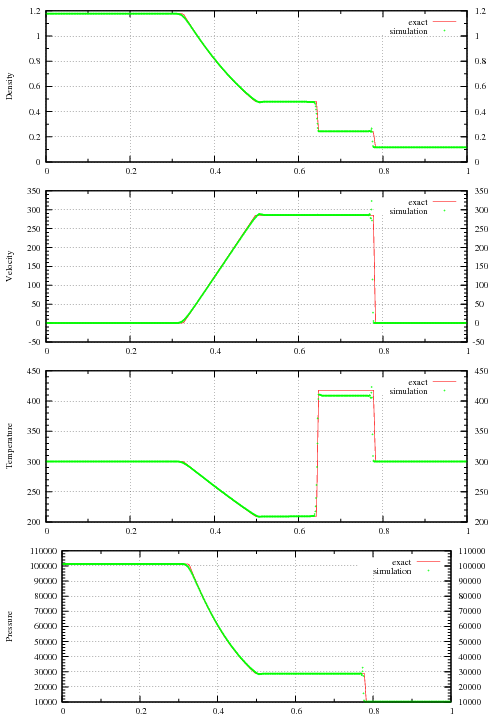
\includegraphics[scale=.85]{shockTube.png}
  \caption{Shock tube results at time $t = 5msec$}
  \label{results.ST}
  \end{figure}
\newpage

%__________________________________SHOCKTUBE AMR

\section*{\center Shock Tube with AMR}
 
\subsection*{\underline{Simulation Specifics}}
\begin{description} 
\footnotesize
\item [Component used:] \hfill ICE
\item [Input file name:] \hfill shocktube\_AMR.ups
\item [Command used to run input file:]\hfill sus inputs/UintahRelease/ICE/shocktube\_AMR.ups
\item [Postprocessing command:]\hfill \\
inputs/UintahRelease/ICE/plot\_shockTube\_AMR shockTube\_AMR.uda y
This will generate a postscript file shockTube\_AMR.ps

\item [Simulation Domain:]\hfill    1 x .001 x .001 m
\item [Cell Spacing:]\hfill 
10 x 1 x 1 mm (Level 0)\\
2.5 x 1 x1 mm (Level 1)\\
0.625 x1 x1 mm (Level 2)

\item [Example Runtimes:] \hfill \\
 2ish minutes   (1 processor, 2.66 GHz Xeon)

\item [Physical time simulated:] \hfill 0.005 sec.

\end{description}

\section*{\underline{Results}}
Figure \ref{results.ST.AMR} shows a comparison of the exact versus simulated results at time $t = 5msec$.
\begin{figure}
  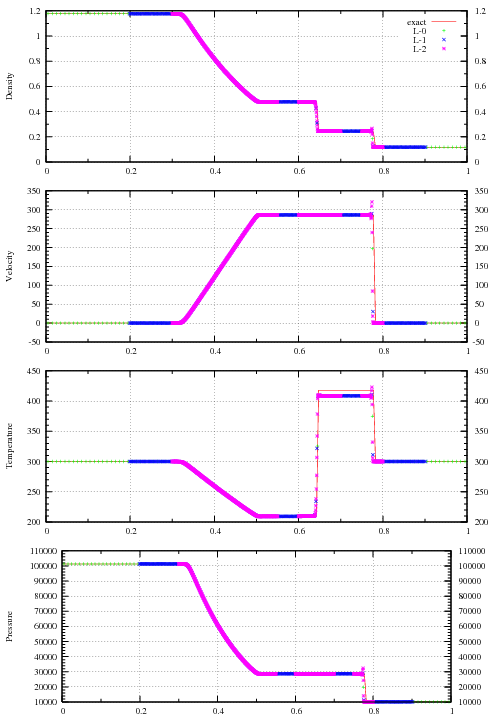
\includegraphics[scale=.85]{shockTube_AMR.png}
  \caption{Shock tube results at time $t = 5msec$}
  \label{results.ST.AMR}
  \end{figure}
\newpage

%__________________________________riemann2D

\section*{\center 2D Riemann Problem with AMR}
\subsection*{\underline{Problem Description}}
In two-dimensional Riemann problems there 15 different solutions that combine rarefaction waves, shock waves and a slip line or contact discontinuities \cite{ref:schulz_collins_glaz, ref:Liska_Wendroff}.  Here we simulate 4 slip lines that form a symmetrical single vortex turning counter clockwise. At time $t=0$ the computational domain is divided into four quadrants by the lines $x = 1/2, y=1/2$  The initial condition for $V=(p, \rho, u, v)$ in the four quadrants are $V_{ll}=(1, 1, -0.75, 0.5), V_{lr}=(1, 3, -0.75,-0.5), V_{ul}=(1,2,0.75,0.5), V_{ur}=(1,1,0.75,-0.5)$ where, $p$ is pressure, $\rho$ is the density of the polytropic gas, $u$ and $v$ are the $x$ and $y$ component of velocity.
\subsection*{\underline{Simulation Specifics}}
\begin{description} 
\footnotesize
\item [Component used:] \hfill ICE
\item [Input file name:] \hfill riemann2D\_AMR.ups
\item [Command used to run input file:]\hfill mpirun -np 5 sus inputs/UintahRelease/ICE/riemann2D\_AMR.ups
\item [VisIT session file:]\hfill inputs/UintahRelease/ICE/riemann2D.session
\item [Simulation Domain:]\hfill    0.96 x 0.96m x 0.1 m
\item [Cell Spacing:]\hfill \\ 
40  x 40  x 1 mm (Level 0)\\
10  x 10  x 1 mm (Level 1)\\
2.5 x 2.5 x 1 mm (Level 2)

\item [Example Runtimes:] \hfill \\
 5ish minutes   (5 processors, 2.66 GHz Xeon)
\item [Physical time simulated:] \hfill 0.3 sec.
\end{description}

\section*{\underline{Results}}
Figure \ref{fig:riemann2D} shows a flood and line contour plot(s) of the density of the gas at 0.03sec.
\begin{figure}
  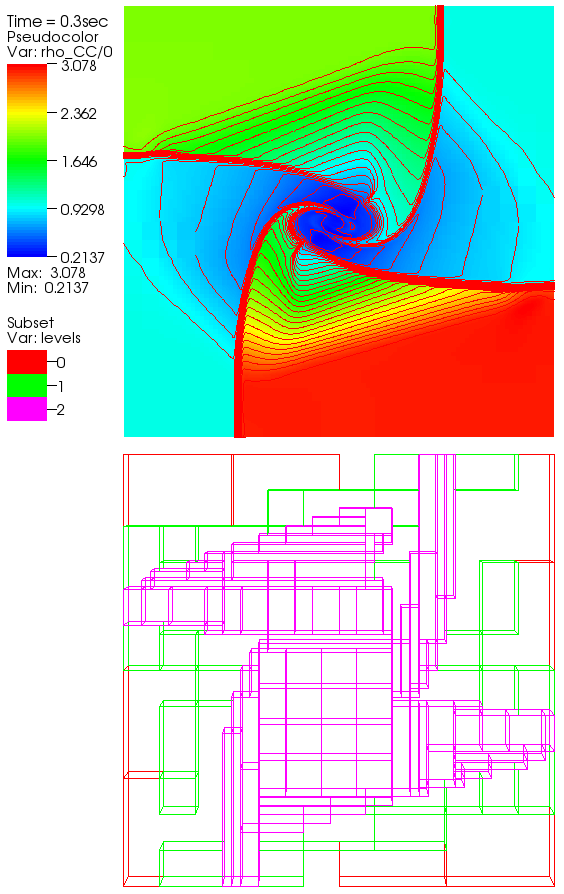
\includegraphics[scale=.6]{riemann2D.png}
  \caption{Contour plot of density for the 2D Riemann problem at time $t = 0.3sec$.  Bottom plot shows the outline of the patches on the 3 levels.}
  \label{fig:riemann2D}
  \end{figure}
\newpage

%__________________________________Single level blast wave

\section*{\center BlastWave 2D}
\subsection*{\underline{Problem Description}}
The Sedov-Taylor blastwave problem is a standard compressible flow problem
that has been used by many as a validation test case.  At time $t=0$ there
is a small region of gas at the center of the domain at a relatively high
temperature and pressure.  The expansion of high pressure gas forms a
spherical blast wave that expands into surrounding atmosphere.
\subsection*{\underline{Simulation Specifics}}
\begin{description} 
\item [Component used:] \hfill ICE
\item [Input file name:] \hfill blastWave.ups
\item [Command used to run input file:]\hfill sus blastWave.ups
\item [Visualization net file:]\hfill blastWave\_1L.srn\\


\item [Simulation Domain:]\hfill    1 x 1 x .05 m
\item [Cell Spacing:]\hfill \\ 
5 x 5 x 50 mm (Level 0)


\item [Example Runtimes:] \hfill \\
 9ish minutes   (1 processor, 2.66 GHz Xeon)

\item [Physical time simulated:] \hfill 0.9e-3sec.

\end{description}

\section*{\underline{Results}}
Figure \ref{results.BW} shows a comparison of the exact versus simulated
results at time $t = 5msec$.

\begin{figure}
  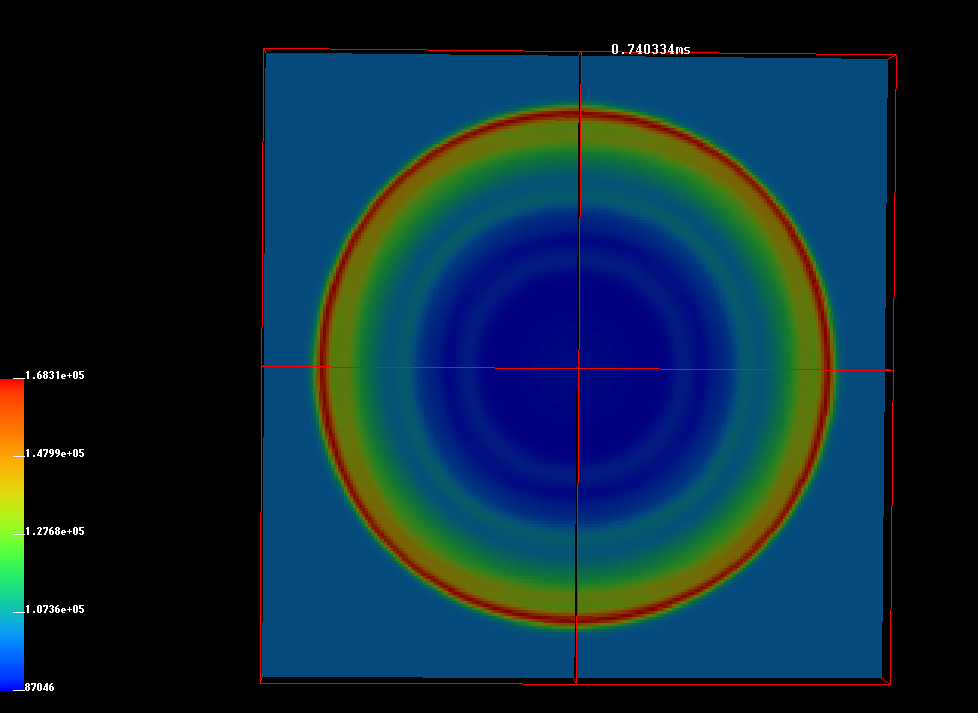
\includegraphics[scale=.5]{blastWave.png}
  \caption{Pressure field at time $t = 0.74msec$}
  \label{results.BW}
  \end{figure}
\newpage

%__________________________________AMR blast wave

\section*{\center BlastWave AMR}
\subsection*{\underline{Simulation Specifics}}
\begin{description} 
\item [Component used:] \hfill ICE
\item [Input file name:] \hfill blastWave.ups
\item [Command used to run input file:]\hfill sus blastWave\_AMR.ups
\item [Visualization net file:]\hfill blastWave\_1L.srn\\


\item [Simulation Domain:]\hfill    1 x 1 x .05 m
\item [Cell Spacing:]\hfill \\ 
20 x 20 x 50 mm (Level 0) 
5 x 5 x 50 mm (Level 1)


\item [Example Runtimes:] \hfill \\
 9ish minutes   (1 processor, 2.66 GHz Xeon)

\item [Physical time simulated:] \hfill 0.9e-3sec.

\end{description}

\section*{\underline{Results}}
Figure \ref{results.BW.AMR} shows the pressure field and an outline of the
individual patches on levels 0 \& 1.  This simulation shows the adaptive
mesh capabilities of ICE and the UCF.
\begin{figure}
  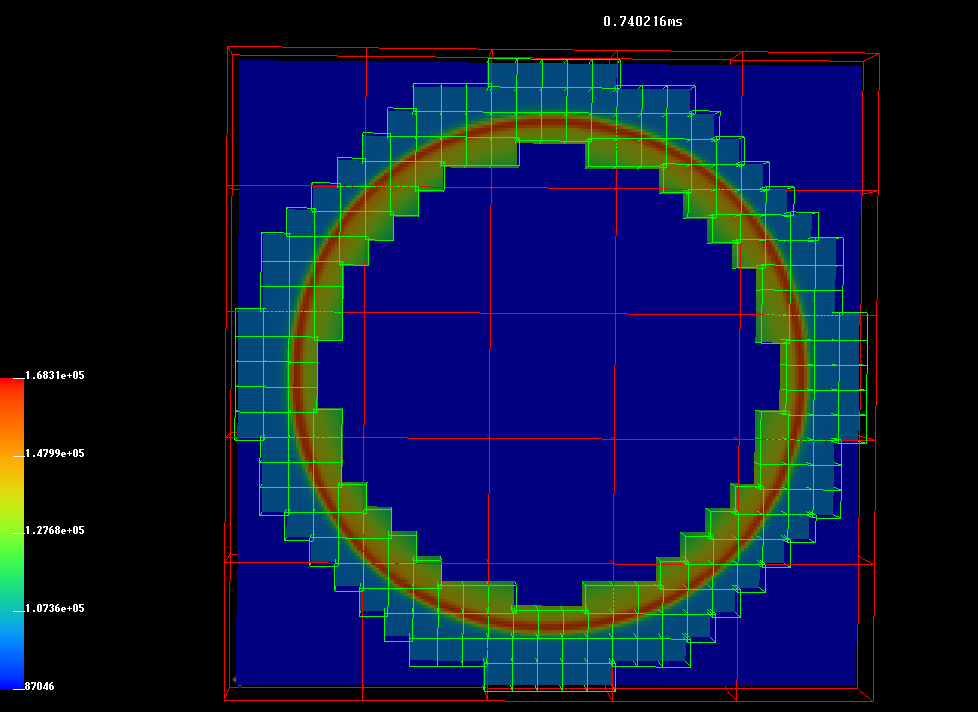
\includegraphics[scale=.5]{blastWave_AMR.png}
  \caption{Pressure field at time $t = 0.74msec$.  The individual patches on levels 0 \& 1 are shown.}
  \label{results.BW.AMR}
  \end{figure}
Good agreement between the single level results (Fig. \ref{results.BW}) and the AMR results (Fig.
\ref{results.BW.AMR}) is shown.
\newpage

%__________________________________CH4 fire

\section*{\center Methane Flame}
\subsection*{\underline{Problem Description}}
At $t=0$ Methane gas begin flowing from a $1m$ hole in the floor of the
computational domain at a velocity of $1m/s$.  The methane mixes with the
surrounding air, ignites and forms a puffing fire.  The main assumptions in
this simulation are a) that the chemical reactions are taking place infinitely
fast (equilibrium chemistry model) and b) that there is no radiative heat
loss from the product gases.
\subsection*{\underline{Simulation Specifics}}
\begin{description} 
\item [Component used:] \hfill ICE
\item [Input file name:] \hfill CH4\_fire.ups
\item [Command used to run input file:]\hfill sus CH4\_fire.ups \\
Note you must have a link to the {\tt inputs} directory in the save directory as sus.  A table needed
by the combustion model is inside the {\tt inputs} directory.
\item [SCIRun visualization net file:]\hfill 3DFire\_Vol.srn \\


\item [Simulation Domain:]\hfill    5 x 5 x 5 m
\item [Cell Spacing:]\hfill \\ 
3.3 x 3.3 x 3.3 cm (Level 0)


\item [Example Runtimes:] \hfill \\
 8 hours   (64 processor, 2.66 GHz Xeon)

\item [Physical time simulated:] \hfill 3.4sec.

\end{description}

\section*{\underline{Results}}
Figure \ref{results.CH4} shows a 3D view of the initial puff just before it leaves the computational
doman.  
\begin{figure}
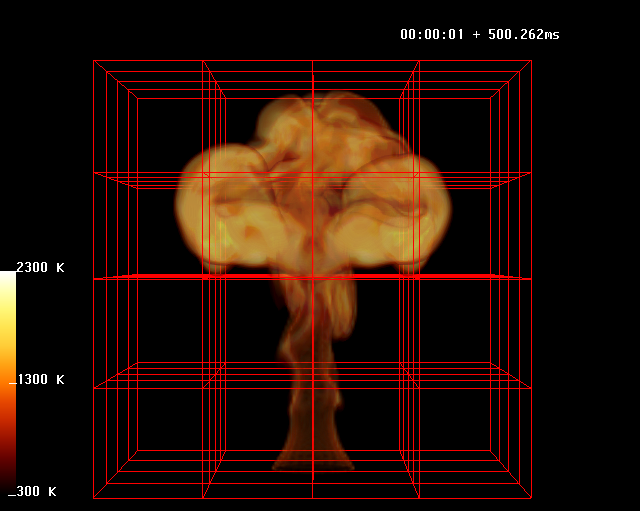
\includegraphics[scale=.66]{3DFire.png}
\caption{Temperature field at time $t = 1.5 sec$}
\label{results.CH4}
\end{figure}
\newpage


\subsection{References}
\bibliographystyle{plain}
\bibliography{ice}


